\documentclass{llncs}
%\documentclass[letterpaper, 10pt]{article}


\usepackage{graphicx}
\usepackage{subfig}
\usepackage{url}
\usepackage{listings}
\usepackage{authblk}


\newcommand{\TODO}[1]{\textbf{TODO:} \emph{#1} }
\newcommand{\NOTE}[1]{\textbf{NOTE:} \emph{#1} }
% Uncomment the following lines to remove TODO and NOTE labels
\renewcommand{\TODO}[1]{}
\renewcommand{\NOTE}[1]{}

\def\GenoM{G\textsuperscript{en}oM~}

\lstset{language=Python, basicstyle=\scriptsize, tabsize=4}



\title{\LARGE \bf Evaluation of Robotics Software Using the MORSE Simulator}

%%%%%%%%%%%%%%%%%%%%%%%%%%%%%%%%%%%%%%%%%%%%%
% Standard author list
%%%%%%%%%%%%%%%%%%%%%%%%%%%%%%%%%%%%%%%%%%%%%
%\author[1]{Gilberto Echeverria \thanks{gechever@laas.fr}}
%\author[1]{S{\'e}verin Lemaignan \thanks{slemaign@laas.fr}}
%\author[1]{Arnaud Degroote \thanks{adegroot@laas.fr}}
%\author[2]{Michael Karg\thanks{kargm@in.tum.de}}
%\author[3]{Pierrick Koch\thanks{pierrick.koch@gmail.com}}
%\author[4]{Charles Lesire-Cabaniols\thanks{charles.lesire@onera.fr}}
%\affil[1]{LAAS-CNRS, Toulouse, France}
%\affil[2]{TUM, Munich, Germany}
%\affil[3]{IRD, Hanoi, Vietnam}
%\affil[4]{ONERA, Toulouse, France}
%
%\renewcommand\Authands{ and }

%%%%%%%%%%%%%%%%%%%%%%%%%%%%%%%%%%%%%%%%%%%%%
% LLNCS author list
%%%%%%%%%%%%%%%%%%%%%%%%%%%%%%%%%%%%%%%%%%%%%
\author{Gilberto Echeverria\inst{1}\thanks{\email{gechever@laas.fr}}
    \and S{\'e}verin Lemaignan\inst{1}\thanks{\email{slemaign@laas.fr}}
    \and Arnaud Degroote\inst{1}\thanks{\email{adegroot@laas.fr}}
    \and Simon Lacroix\inst{1}\thanks{\email{slacroix@laas.fr}}
    \and Michael Karg\inst{2}\thanks{\email{kargm@in.tum.de}}
    \and Pierrick Koch\inst{3}\thanks{\email{pierrick.koch@gmail.com}}
    \and Charles Lesire-Cabaniols\inst{4}\thanks{\email{charles.lesire@onera.fr}}
}

\institute{
	    CNRS, LAAS, 7 avenue du colonel Roche, F-31077 Toulouse, France
	    Universit{\'e} de Toulouse, UPS, INSA, INP, ISAE, LAAS,
	    F-31077 Toulouse, France
        \and
        Institute for Advanced Study, Technische Universität M\"{u}nchen, 
	Lichtenbergstrasse 2a, D-85748 Garching, Germany
        \and
        IRD,
        Hanoi, Vietnam
        \and
       	ONERA Centre de Toulouse -- DCSD, 2 avenue {\'E}douard Belin,
    	F-31055 Toulouse, France
}


\begin{document}
\maketitle

\begin{abstract}
  MORSE is a robotics simulation software developed with the collaboration of
  researchers in several universities. It is a tool to test robotics software
  and algorithms in fairly complex environments. The simulations allow a medium
  to high level of abstraction, to enable researchers to focus on the solution
  of complex tasks.  This is accomplished by connecting directly with the
  robotics software using various existing middlewares, such as ROS, YARP and
  others.
  MORSE makes use of the Blender 3D software to produce realistic looking
  environments with physics simulation.  After three years of development,
  MORSE is a mature tool with a large collection of components.
  Among the innovative features of MORSE are: middleware overlays that make
  integration with external software transparent, distributed multi-node
  simulation for complex scenes and a human avatar that can interact with
  the robots in simulation.
  We present in this paper the current state of the simulator as well as the
  use cases where it has been used to validate several robotics experiments.
\end{abstract}

%%%%%%%%%%%%%%%%%%%%%%%%%%%%%%%%%%%%%%%%%%%%%%%%%%%%%%%%%%%%%%%%%%%%%%
\section{Introduction}
\label{section:introduction}

Computer simulations are today an essential component in robotics research.
Almost every sort of experiment can be validated in simulation before executing
it on real robots.  For this validation to be useful, the simulation must
provide enough fidelity with respect to the real world, within the requirements
of the experimentation.
Creating a fully realistic simulation would be near impossible, since there are
too many aspects that it would need to handle. This is why there are many
simulators with various capacities, each one created to comply with specific
requirements.

The MORSE simulator we present here is meant as a tool that can be used to test
and evaluate very complex robots performing advanced missions in real life
environments. It does not focus on lower level control of the robot, or the
specific mechanics of its components. In turn, it can provide all the
functionality necessary to evaluate the algorithms that control a robot during
the execution of a mission.


%%%%%%%%%%%%%%%%%%%%%%%%%%%%%%%%%%%%%%%%%%%%%%%%%%%%%%%%%%%%%%%%%%%%%%
\section{Competing Simulators}
\label{section:othersims}

There are a number of other robotics simulators available, both commercial and
free. We evaluate here the ones whose functionality is most similar to MORSE:

The Player/Stage/Gazebo suite \cite{psg-1232} is very well known in robotics.
It is a full set of tools that include the Player communication layer and two
very integrated simulators: Stage \cite{Gerkey03theplayer/stage} is basically a
2D simulator optimised for navigation on flat and closed environments.
One of its advantages is the capability to handle very large numbers of
simplified robots \cite{springerlink:10.1007/s11721-008-0014-4}. However, it is
not ideal for more complex scenarios, specially in 3D space.  The more recent
Gazebo \cite{Koenig04designand} was developed to cover these shortcomings.
It has received an important boost in its development with its integration
into the ROS platform.

The USARSim \cite{usarsim-4209284} shares many design concepts with MORSE. It
was initially developed as a simulator for search and rescue operations, uses
the Unreal Engine gaming platform and is built with the concept of modular
components. It is widely used as an evaluation tool for the well known RoboCup
competitions. However, it uses a custom interface to communicate with external
software and does not support some of the most common robotics middlewares.

Another popular robotics simulator is Webots \cite{Webots04}, which is a
commercial product. It provides a full programming environment to create
customised robots and environments, but its interface is complex to use when
creating new components and robots.
It also has an integrated code editor, but the control programs created in it
must then be converted and transferred to the final robot platform.


% Genom \cite{MALLET-2011-599677},




%%%%%%%%%%%%%%%%%%%%%%%%%%%%%%%%%%%%%%%%%%%%%%%%%%%%%%%%%%%%%%%%%%%%%%
\section{MORSE Overview}
\label{section:overview}

% Morse \cite{5980252}

One of the characteristics of MORSE is that it does not deal with the super
realistic simulation of each of the robotics components. Instead, it uses
simplified components that can nevertheless provide the same data as their real
world counterparts. This simplification not only allows the simulation to be
faster, but also permits the robotics researchers to concentrate on testing
higher level algorithms for the completion of the desired tasks.

MORSE is developed as a library of Python scripts that run on the Blender Game
Engine (BGE).  The BGE offers a powerful environment for a graphical
application and uses the Bullet Physics Engine.
Objects in the BGE can be completely configured, from physics properties (like
mass, friction coefficients and collision bounding boxes) to event and
behaviour scripts using Python


The simulation is organised as a main core of control functionality that sets
up and coordinates the events in the BGE, and a collection of components that
can be used to assemble a robot. Additionally, there is a variety of
communication tools that allow each of the MORSE components to connect with
external robotics software via various middlewares.
MORSE has support for some of the most commonly used robotics middlewares,
including ROS \cite{ros-288}, Pocolibs and YARP \cite{metta|ars06}.
Other middlewares are constantly being added, mainly driven by the needs of new
users. This process is simple, as existing middleware bindings can be used as a
template for the new ones.

Individual components are minimalistic in their functionality and  completely
middleware agnostic. They store the important data that needs to be shared
outside MORSE in a Python dictionary called \texttt{local\_data}. When a
simulation scene is created, the components are linked to middlewares as
specified in the configuration script, and the necessary functionality is added
to the components to be able to transmit/receive data through the middleware.
During a simulation, each component performs its expected task and exchanges
the \texttt{local\_data} with the external software.

The data employed by the components can also be altered through the use of
components called \emph{modifiers}. These provide access to the
\texttt{local\_data} to add noise or change the data as required. For instance,
transforming the coordinate frame used by Blender into the Universal Transverse
Mercator (UTM) coordinate system.

MORSE can be easily extended by adding new components that inherit from the
existing base classes. All components are programmed in Python, since this is
the language that Blender uses for its scripts. However, when coding components
that require a faster processing time, they can be implemented in C/C++, and
then use SWIG to create interfaces that can be included in Python.

\subsection{Blender Integration}
\label{section:blender}

Being based on the Blender 3D \cite{blender|web} modelling software, any
object, robot or environment can be created and immediately be made available
to use in MORSE.
Many other file formats for 3D models can also be imported directly into
Blender, further increasing the range of components that can be used.
The high level of graphical detail is specially useful for realistic looking
simulations, and very important when doing image processing from simulated
video cameras.
Figure \ref{fig:models} shows the modelling capabilities of Blender being used
to create the MORSE robots and environments. The right image shows also the
view obtained from a camera mounted on the helicopter robot.

\begin{figure}[h!]
\centering
\begin{tabular}{cc}
 %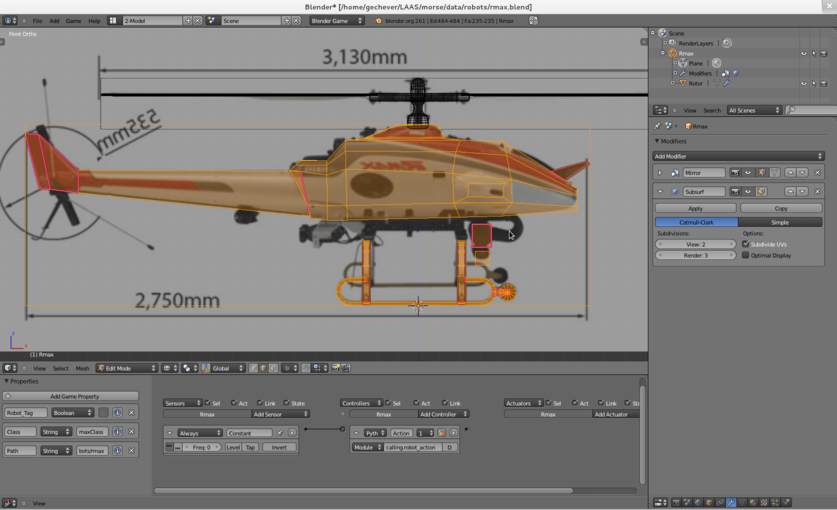
\includegraphics[width=0.475\textwidth]{pics/MORSE-rmax_mesh.png} &
 %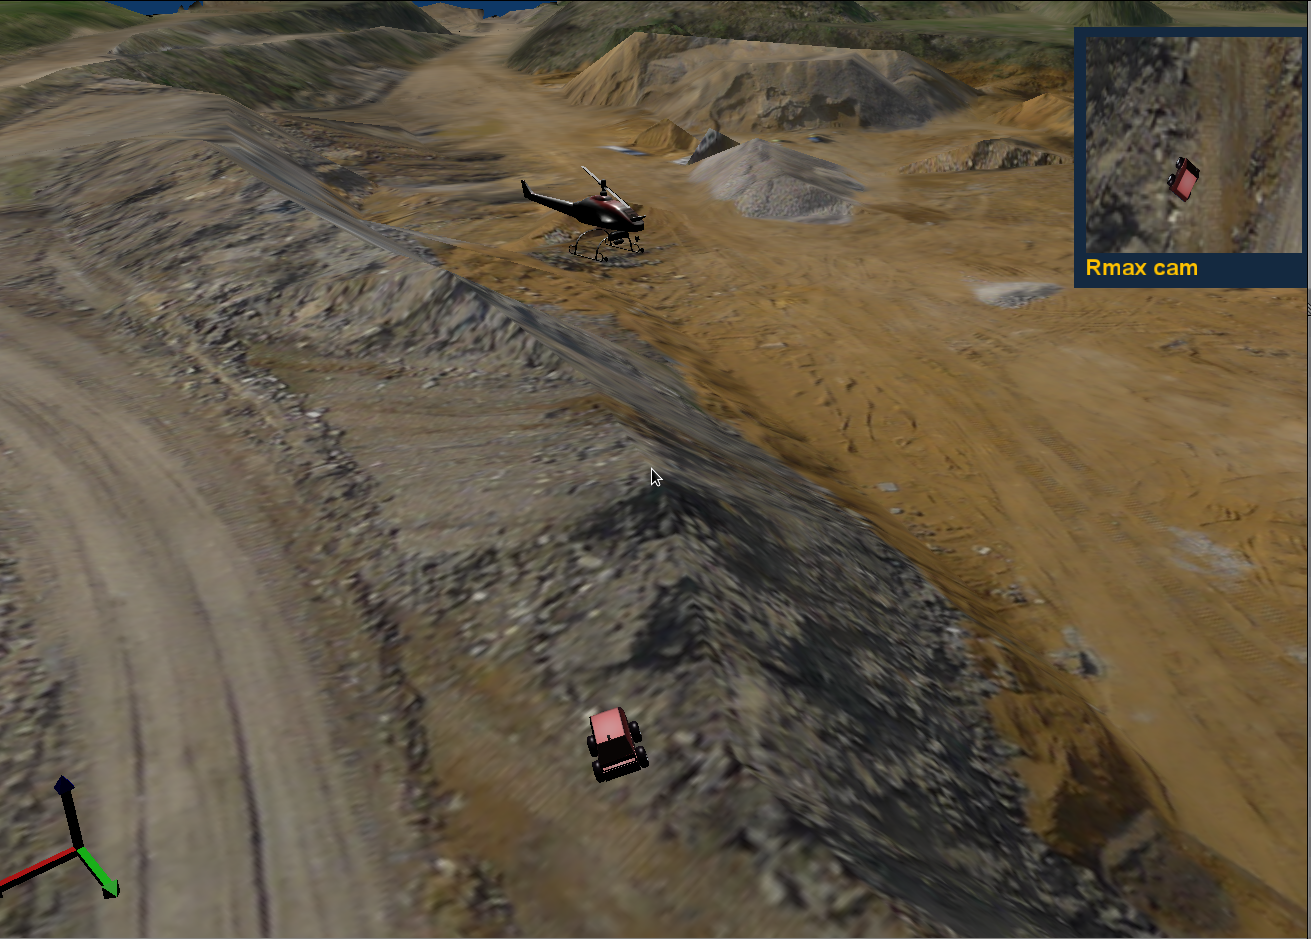
\includegraphics[width=0.475\textwidth]{pics/MORSE-quarry_ok-1.png}
 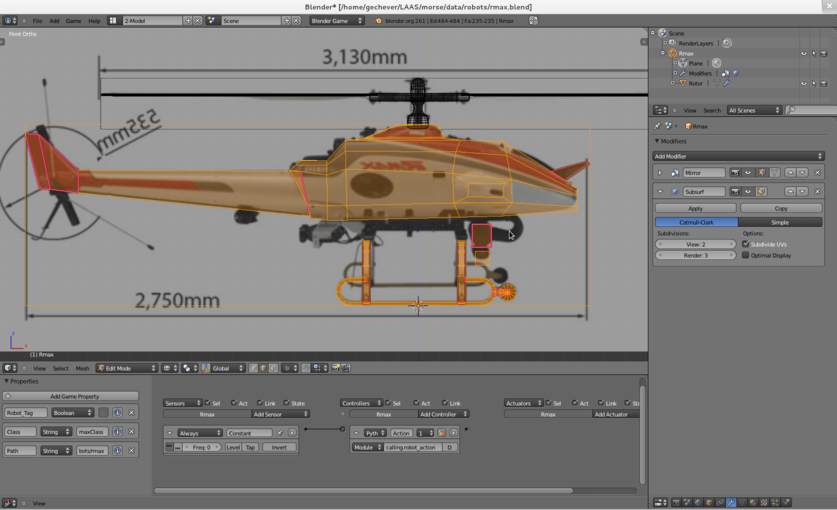
\includegraphics[height=1.5in]{pics/MORSE-rmax_mesh.png} &
 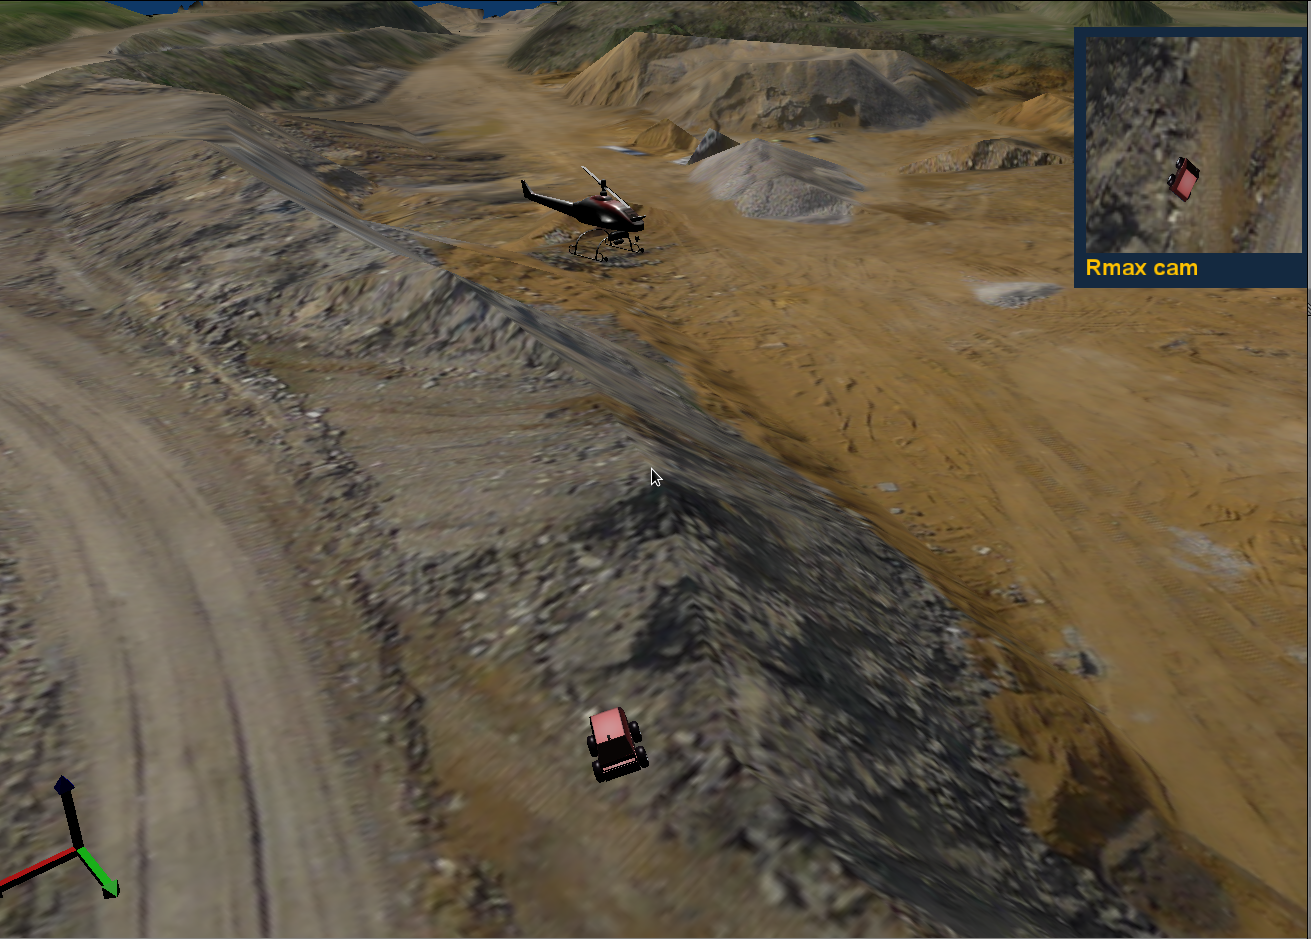
\includegraphics[height=1.5in]{pics/MORSE-quarry_ok-1.png}
\end{tabular}
\caption{Left: Modelling of an R-Max robotic helicopter. Right: Robots on a
    terrain imported from a Digital Elevation Map, using a Python plug-in
    for Blender developed along with MORSE.}
\label{fig:models}
\end{figure}

Experiments in \emph{field robotics} benefit from having an accurate
representation of the terrain where the real robots are expected to perform.

%one robot in large outdoors environments. The terrain should not be initially
%known to the robots, so they are expected to explore and navigate autonomously
%as they carry out their mission.
%The robots do not directly affect the environment, but have a large number of
%sensors that allow them to navigate and accomplish specific objectives.


\subsection{Component Library and Scene Construction}
\label{section:components}

To be as versatile as possible, MORSE consists of a collection of components
that can be used to construct robots with various configurations. The
components are classified as:

\begin{itemize}
  \item Robots in MORSE are mostly just the physical representation of the
    robot. They do nothing by themselves, and only define the physical shape
    and properties like mass, friction and collision bounds Most robots in
    MORSE are treated as a box sliding over the surface of the ground. There
    are however a couple of robots with a more realistic wheel physics
    behaviour, where the speed of the wheels can be controlled directly to
    provide the movement of the robot, using the corresponding actuator
    components
  \item Sensors recover data from the simulated world and store it. This is
    done using the Blender predefined interfaces for the GE and Python scripts.
    For example, laser scanners use ray tracing operations, while cameras use
    renders from the perspective of the camera to produce images
  \item Actuators are charged with carrying out actions within the simulated
    world. There are actuators to provide motion to the robots through several
    methods and algorithms, or to control moving parts such as robotic arms or
    pan-tilt units
\end{itemize}

Additionally, MORSE provides a is a set of Python functions to create and
configure all MORSE simulation scenarios. This tool is know as the
\emph{Builder API}. It completely hides the interface of Blender from the user,
so that those unfamiliar with Blender can directly configure MORSE using Python
scripts. The API offers new classes to create robots, sensors and actuators, as
well as changing any of the parameters used by these components, and including
additional objects (furniture, obstacles, etc.). Middleware bindings of
each component can also be specified in the same script.



\subsection{Multi-node Simulation}
\label{section:multinode}

The simulation of multiple robots in the complex environments permitted by
MORSE is very demanding on computational resources, particularly the
display of the graphics. MORSE offers the possibility of running multiple
instances of the same simulation scenario in separate computers, but
coordinated by a central server program, called the \emph{multi-node
manager}. While all nodes show all of the robots, each node will only
be charged with processing the control of a few robots. The movements
of robots and specific objects in one node are sent to the multi-node
manager, which in turn collects the updated positions across all nodes
and redistributes the information, so that all nodes can immediately
reflected the changes.  The multi-node server is also charged with
synchronising the time and events across all nodes. It can also be used
to slow down the simulation. However, at the current time it is not
possible to accelerate the simulation speed.

This functionality was developed for applications that require a large amount
of robots. Our use case is another outdoors robotics project: \emph{Rosace}
\cite{springerlink:10.1007/978-3-642-12384-9_18,springerlink:10.1007/978-3-642-28786-2_32}.
Its main objective is the coordination of robotic agents in search and rescue
operations in the case of a disaster. In this scenario, terrestrial robots must
be able to locate human victims, provide support for the victims and avoid
dangerous areas. The robots in the team are to be equipped with different
payloads, and take autonomous decisions on which of them should perform
different tasks in the mission, such as searching, providing a communications
relay, and helping victims directly.

To handle such large groups of robots, only a few are directly controlled by
each simulation node. The multi-node manager is then charged with synchronising
the positions of all the robots and the victims as well.


%MORSE also permits giving some basic behaviour to the simulated human victims,
%by scripting movement patterns and allowing them to visually show their
%injured or healthy status by using different colours.



\subsection {Middleware Configurations}
\label{section:middlewares}

Many research laboratories use different interfaces to communicate with their
robots. In order to be usable along with any architecture, MORSE keeps a
separation between components and middlewares.  When a simulation is started,
the bindings between sensors/actuators and middlewares are read from the
configuration script, and it is only then that components ``learn'' how to
communicate with the outside world.
This separation means that any middleware can be integrated with MORSE, by
simply providing the scripts to marshal MORSE data in the expected format.
Middlewares currently supported include ROS, MOOS, Pocolibs, YARP and
TCP/IP sockets.

Another advantage is the possibility of using many different middlewares within
a single simulation scenario. This is exemplified in the \emph{Action project}
\cite{6106782}, which consists on the cooperation between ground
and air robots to locate and follow moving targets.
The robots involved use completely different architectures, but should all
communicate with MORSE.

Tests for this project are done in specific environments, which require
transporting the robots a considerable distance, always being dependant on the
prevailing weather.  The use of
simulation offers the advantage of running the experiments regardless of the
weather, and not having to plan long trips to the actual experimental site.
Simulation also simplifies the execution of test runs, since they can be
restarted from the initial point within seconds.  Future stages of the project
require the coordination of larger teams of heterogeneous robots. The physical
robots required for these stages are not currently available, but simulation
permits for testing of these scenarios in advance.



\subsection{The Human Avatar}
\label{section:human}



For human-robot-interaction scenarios, we were looking for a way to combine the
reactive and sometimes unpredictable behaviour of a human interacting with its
environment with a simulated robot. Therefore the human avatar of the MORSE
simulator has been equipped with an intuitive 
control that enables users to interact with the simulated environment. Inspired
by modern 3D-computer games, the user takes a third-person perspective behind
the human avatar to move around like shown in figure \ref{fig:human_control} on
the left. 
While moving around, the camera tries to avoid the objects and walls placed
between the camera and the human avatar to prevent occlusions.  All objects
that can be interacted with can be displayed by just pressing a key on the
keyboard which is also illustrated in figure \ref{fig:human_control} on the
left. When the user decides to interact with an object, the camera switches to
a first-person perspective and offers an interface showing possible actions the
user can take when pointing to specific objects like shown in figure
\ref{fig:human_control} on the right. Those actions at the moment include
picking up and releasing objects, opening and closing drawers and cupboards and
switching on and off specific objects like a light or an oven. 

\begin{figure}[h!]
\centering
\begin{tabular}{cc}
 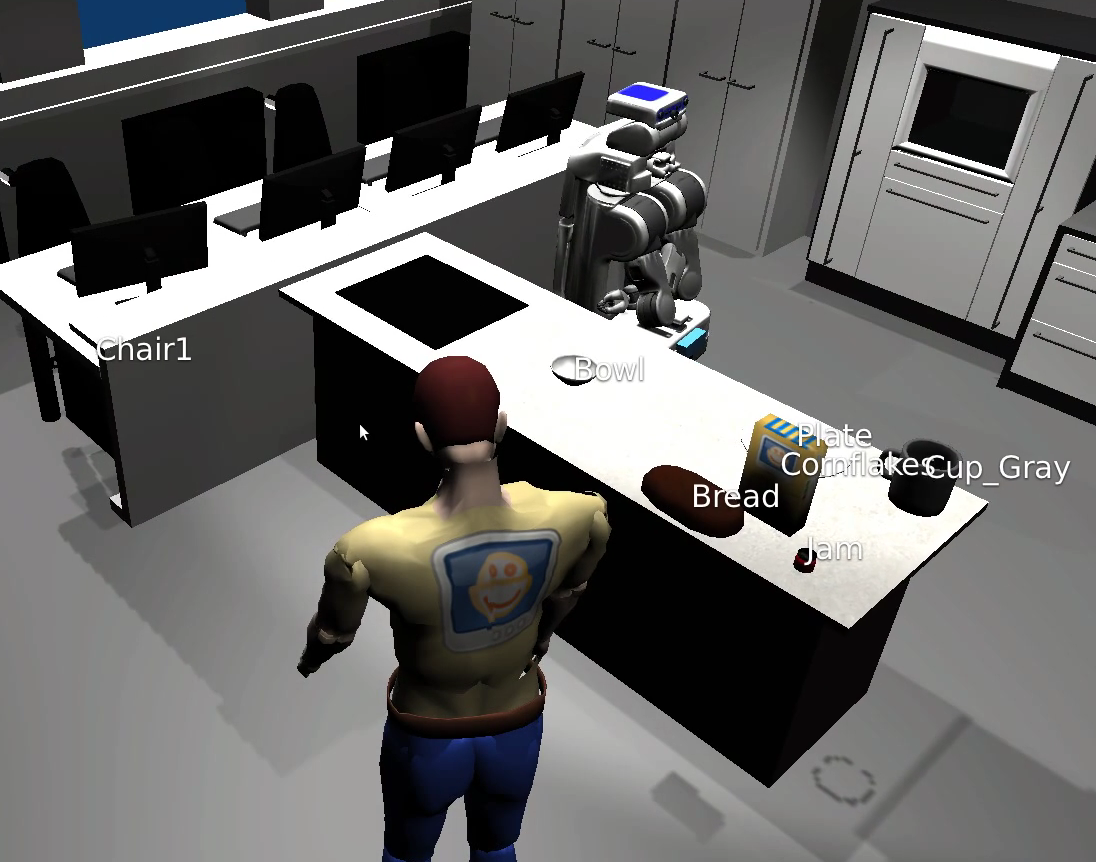
\includegraphics[width=0.475\textwidth]{pics/human_control_1.png} &
 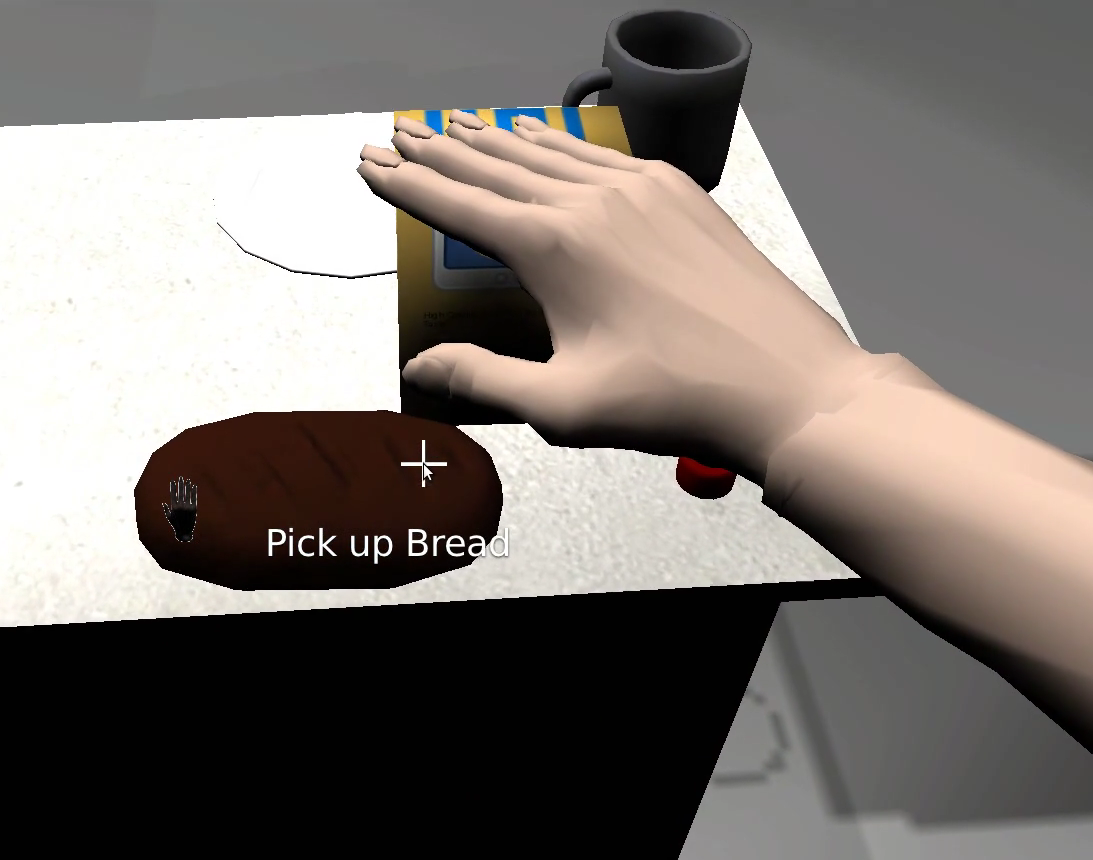
\includegraphics[width=0.475\textwidth]{pics/human_control_2.png}
\end{tabular}
\caption{The left picture shows a third-person view of the human component that
    is used to navigate in the environment. Here objects, that the human can
    interact with, are displayed. The right picture shows the first-person
    perspective of the human avatar that indicates a possible
    ``pick-up-action'' with the bread.}
\label{fig:human_control}
\end{figure}

The avatar can be controlled much like a character in a videogame, using either
the mouse and keyboard or a combination of the Microsoft Kinect and the
Nintendo Wiimote. This computer-game like control enables users to perform
pick- and place actions in simulated worlds using the human component of MORSE
while at the same time, the simulated robot(s) can be controlled the supported
robotic middlewares.

% TODO: Add picture of kinect/wiimote control

The human avatar is meant to be used in \emph{indoor service robotics} scenarios.
In these, complex robots are expected to collaborate with humans to carry out
ordinary household tasks, such as cleaning, serving food or aiding humans to
navigate an environment.
Robots used in these experiments are equipped with one or two arms, and are
capable of grasping objects. They are also expected to react to the actions of
their human collaborator, using video cameras, motion detectors or telemetry to
determine the location, pose and attitude of the human.
This can be done at two different levels of
abstraction. Using the video cameras to recognise the human and its pose can be
done realistically, with the associated computational cost and uncertainties.
Alternatively, the avatar can directly export the position of all of its
joints, and feed them back to the robot, simulating a full motion capture
system and avoiding the processing costs.


In MORSE, the robotic arms can be operated either by control of the end
effector and using Inverse Kinematics (using the iTasc \cite{iTaSC} solver
available in the BGE), or by direct control of the angles at each joint.
The animation of the human avatar also uses IK for its animations.

An example use case in this scenario is the testing and validation of human-aware
navigation planners of service robots in human-centred environments at TU Munich. 
In this case, a simulated human tracking system provides the human pose to the robot
while the robot navigates in the environment in a way that is safe and legible
for the human. For evaluation of human-aware navigation strategies, 
Lichtenth{\"a}ler et al. \cite{lichtenthaeler2012increasing} used MORSE for 
video-based user studies. 
In another project at TU Munich, a simulated kitchen environment is used
to test and evaluate a plan recognition and monitoring system using the 
semantic camera of MORSE as a simulated object recognition system with 
a reactive robot control system.


%%%%%%%%%%%%%%%%%%%%%%%%%%%%%%%%%%%%%%%%%%%%%%%%%%%%%%%%%%%%%%%%%%%%%%
\section{Summary}
\label{section:discussion}


MORSE is developed as an open--source project, the source code can be
downloaded from the GIT repository:
(\url{http://github.com/laas/morse.git})

User documentation and additional information is also available at
(\url{http://morse.openrobots.org})


\subsubsection*{Acknowledgments}
This work has been partially supported by the DGA founded Action project
(\url{http://action.onera.fr}) and the STAE foundation Rosace project
(\url{http://www.fondation-stae.net})

% ---- Bibliography ----
\bibliographystyle{unsrt}
\bibliography{./morseBiblio}
\end{document}
